\section{Arjun Yuda Firwanda(1174008)}
\subsection{Intalasi Map Proxy}
\begin{enumerate}
    \item Gunakan CMD dan Ketikkan pip install map proxy
    \hfill\break
    \begin{figure}[H]
		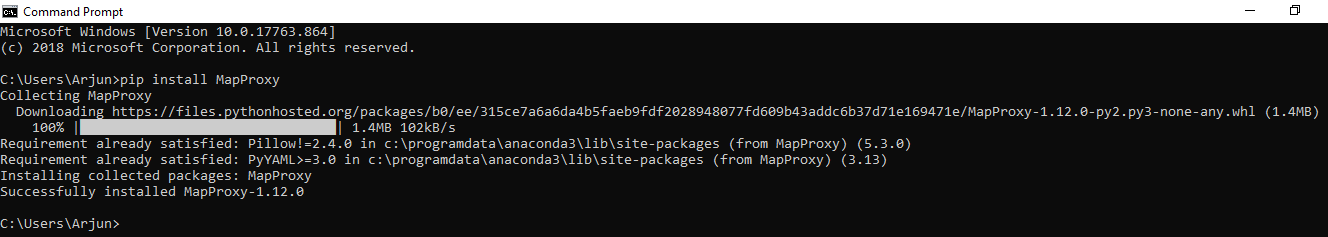
\includegraphics[width=4cm]{figures/1174008/5/1.png}
		\centering
		\caption{Perintah untuk menginstal map proxy}
    \end{figure}
\end{enumerate}

\subsection{Konfigurasi}
\begin{enumerate}
    \item Download filenya terlebih dahulu pada \href{https://github.com/awangga/gede}{Github Pak Rolly}
    \hfill\break
    \begin{figure}[H]
		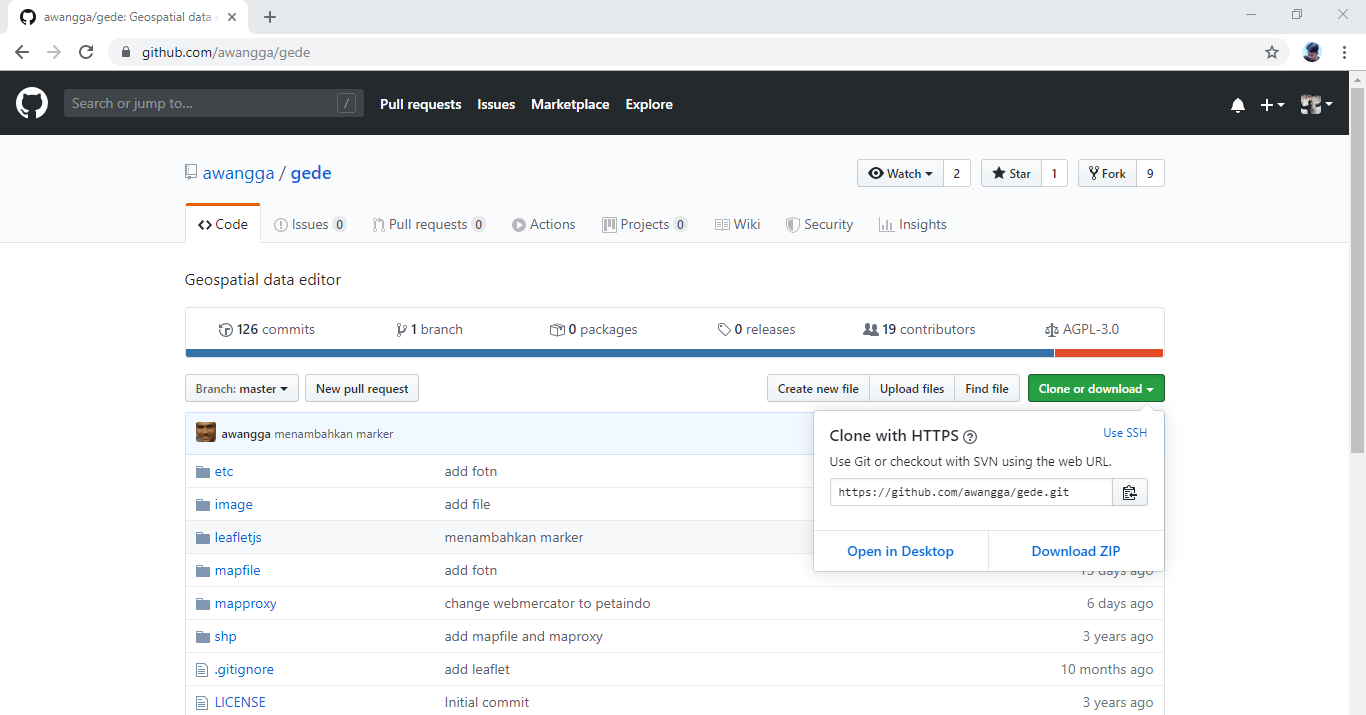
\includegraphics[width=4cm]{figures/1174008/5/2.png}
		\centering
		\caption{Download file untuk melakukan konfigurasi}
    \end{figure}

    \item Setelah didownload kemudian extrak
    \hfill\break
    \begin{figure}[H]
		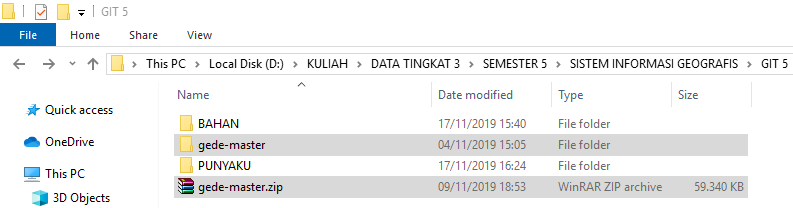
\includegraphics[width=4cm]{figures/1174008/5/3.png}
		\centering
		\caption{Extrack File Gede}
    \end{figure}
    \item Buka file agm.yaml, ubah map sesuai direktori file map, binari ubah sesuai direktori mapserver, working dir ubah sesuai direktori gede-master yang sebelumnya di download.
    \hfill\break
    \begin{figure}[H]
		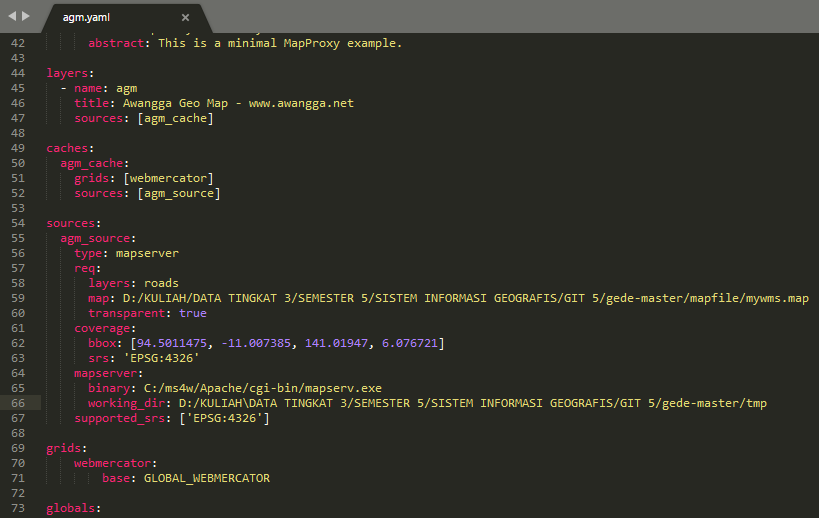
\includegraphics[width=4cm]{figures/1174008/5/4.png}
		\centering
		\caption{Ubah binary dan working dir}
    \end{figure}

    \item Buka Anaconda Promt sebagai administrator, install pyproj, conda install pyproj
    \hfill\break
    \begin{figure}[H]
		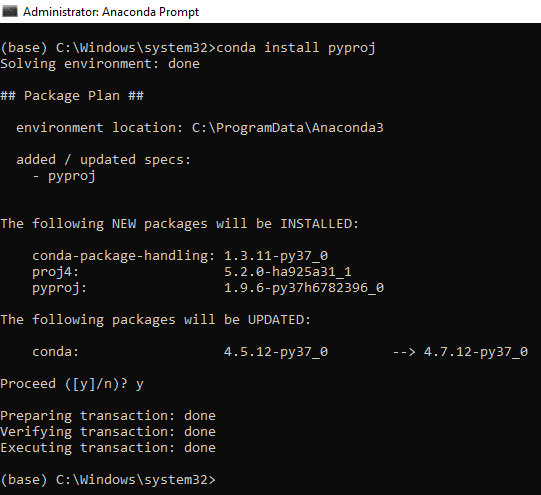
\includegraphics[width=4cm]{figures/1174008/5/5.png}
		\centering
		\caption{Install Pyproj}
    \end{figure} 

\end{enumerate}

\subsection{Pengujian}
\begin{enumerate}
    \item Untuk melakukan pengujian bisa dengan menggunakan perintah mapproxy-util serve-develop mapproxy.yaml -b 0.0.0.0:8181 pada cmd
    \hfill\break
    \begin{figure}[H]
		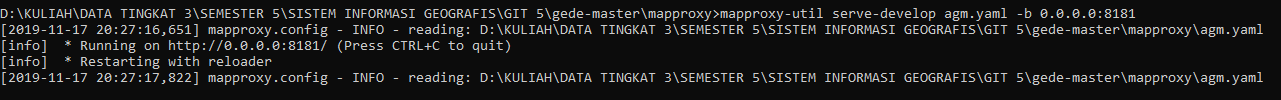
\includegraphics[width=4cm]{figures/1174008/5/6.png}
		\centering
		\caption{Perintah untuk menjalankan mapproxy}
    \end{figure}

    \item Jalankan di browser http://127.0.0.1:8181/
    \hfill\break
    \begin{figure}[H]
		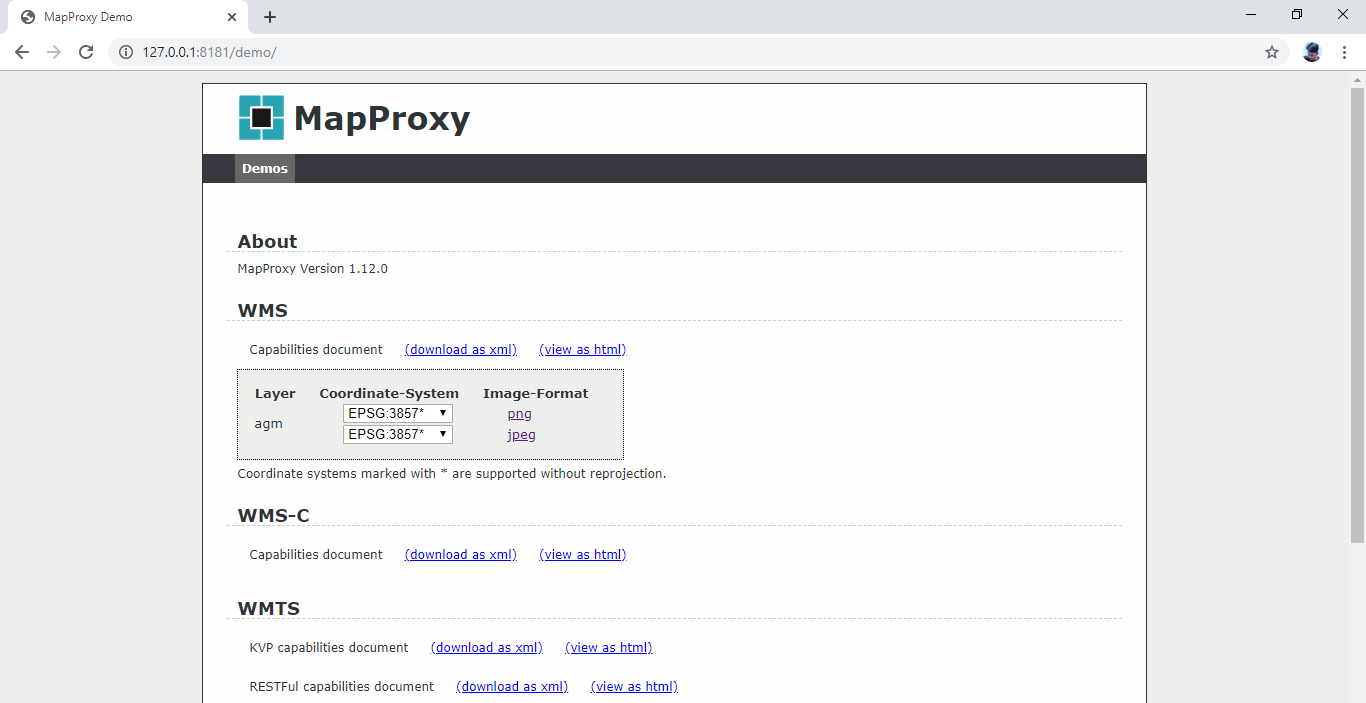
\includegraphics[width=4cm]{figures/1174008/5/7.png}
		\centering
		\caption{Hasil pada Web Browser}
    \end{figure}

\end{enumerate}

\subsection{Link Youtube}
\href{https://www.youtube.com/watch?v=VoWTSqLcKVg&feature=youtu.be}{Klik Disini}